\documentclass[journal]{IEEEtran}

\usepackage{flushend} % For end of document
\usepackage{graphicx,color}
\usepackage[super]{nth}
\usepackage{wrapfig}
\graphicspath{./images/}
\pagestyle{plain}

\title{CS6000 \nth{1} Journal}
\author{Mark Maldonado}
\date{August 2022}

\begin{document}

    \maketitle

    \section{Course Goals}
    \label{sec:Goals}
        \begin{wrapfigure}{L}{0.25\textwidth}
            \centering
            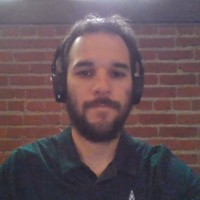
\includegraphics[width=0.25\textwidth]{images/maldonado_profile.jpg}
        \end{wrapfigure}
        My course goals for this class is to learn better habits to conducting research.
        Since I am already doing research in the cybersecurity domain professionally, I would like to discover new ways to conduct research.
        Doing the bear minimum while reading papers and posting on open-source forums will only take you so far for understanding the field of study.
        The ability to inherit multiple ways to investigate the field of study to achieve your research goals is critical to becoming a sound researcher.

        For my PhD I am researching a novel means to deploy and build honeypots by implementing them with a novel architecture and framework.
        The research behind the honeypots will provide improved methods to deceiving malicious attackers from penetrating production networks and attacking the decoys instead.
        Integrating these deployments and intelligence collection with machine learning algorithms will improve the overall network security stature.
        Machine learning will also be used in log aggregation and decision making for humans to approve or deny of autonomous deployment capabilities.

        I intend to build a company out of this research and hope to help improve the global security of enterprise networks.
        This is one of my main goals after completing my PhD amongst other side projects I still intend to complete.
        As a hobby I do a ton of side programming for my family creating multiple gadgets using either arduino or a raspberry pi's.
        Each of my siblings have gotten a small gadget they requested to help with every-day life in their household.

    \section{Related Code Base}
    \label{sec:code}
        I found an open source ecosystem for deploying honeypots using a LAMP stack.
        This software is managed by a group of people and has a decent amount of support for it.
        The software is capable of monitoring and manage the deployed honeypots.
        Their git repository is named \href{https://github.com/honeytrap/honeytrap}{Honeytrap}.


    \bibliography{references}
    \bibliographystyle{IEEEtran}

    \flushend

\end{document}
